
\documentclass{beamer}

\usepackage{graphicx}
\usepackage{amsmath}
\usepackage{amssymb}
\usepackage{subfiles}
\begin{document}
	
	%=========================================================== %
	\begin{frame}
		\begin{figure}
			\centering
			
\includegraphics[width=0.6\linewidth]{rlogo}
		\end{figure}
		\large
		\[ \mbox{"10 R packages that I wish I knew about earlier" - revisited} \] \bigskip
		
	\end{frame}
	%================================================================ %
\begin{frame}
	\begin{figure}
		\centering
		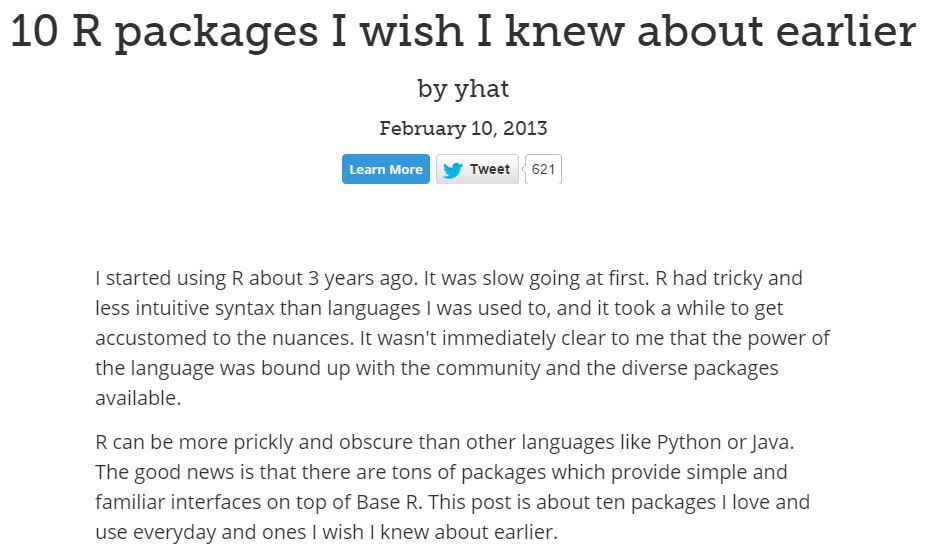
\includegraphics[width=1.05\linewidth]{tenpackintro01}
		
	\end{figure}
	
\end{frame}
%================================================================ %
\begin{frame}
	\begin{figure}
		\centering
		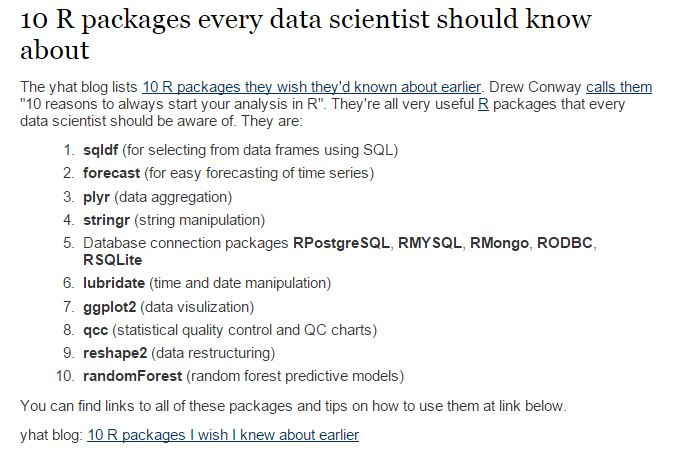
\includegraphics[width=1.05\linewidth]{tenpackintro02}
		
	\end{figure}
	
\end{frame}
%================================================================ %
\begin{frame}
	\begin{figure}
		\centering
		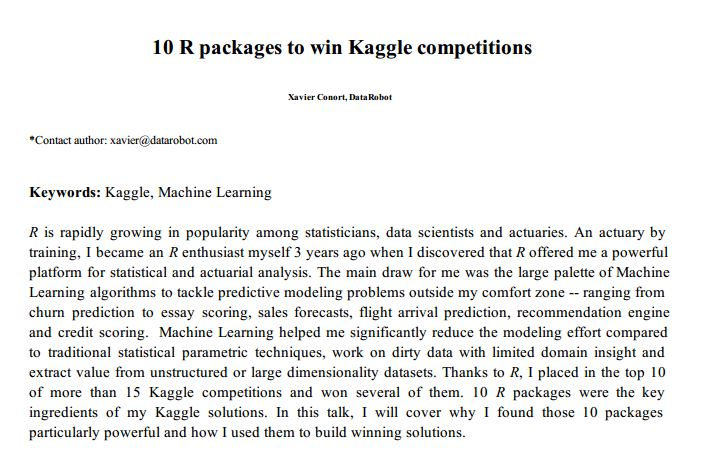
\includegraphics[width=1.05\linewidth]{tenpackintro04}
		
	\end{figure}
	
\end{frame}
%================================================================ %
\begin{frame}
	\begin{figure}
		\centering
		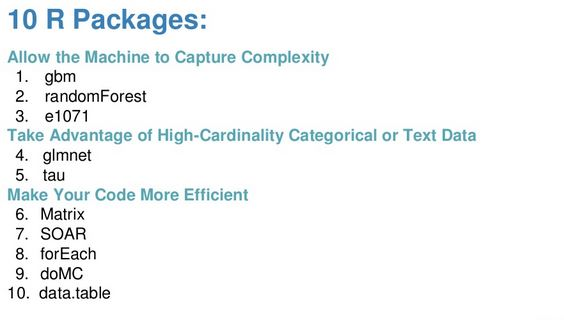
\includegraphics[width=1.05\linewidth]{tenpackintro03}
		
	\end{figure}
	
\end{frame}

%================================================================ %
\begin{frame}
	\begin{figure}
		\centering
		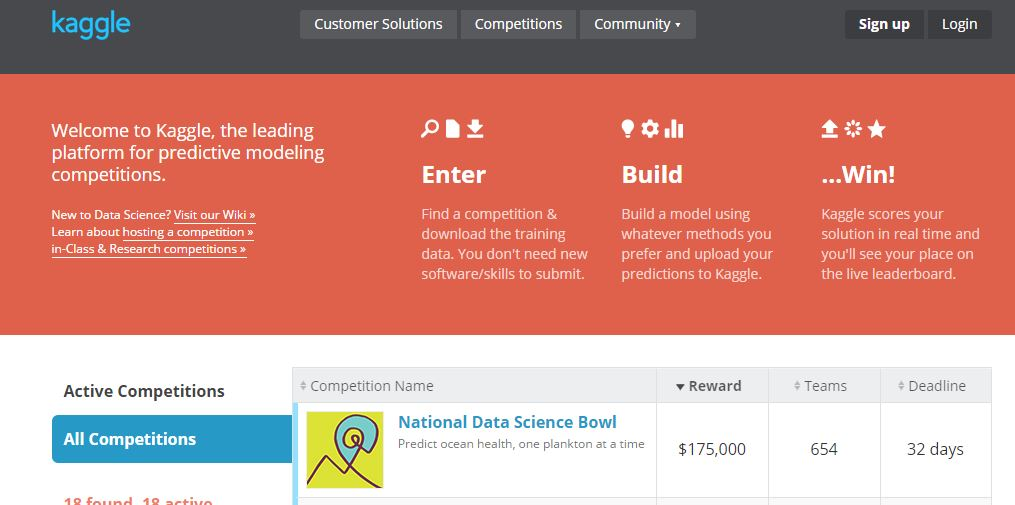
\includegraphics[width=1.05\linewidth]{tenpackintro05}
		
	\end{figure}
	
\end{frame}
%================================================================ %
\begin{frame}
	\begin{figure}
		\centering
		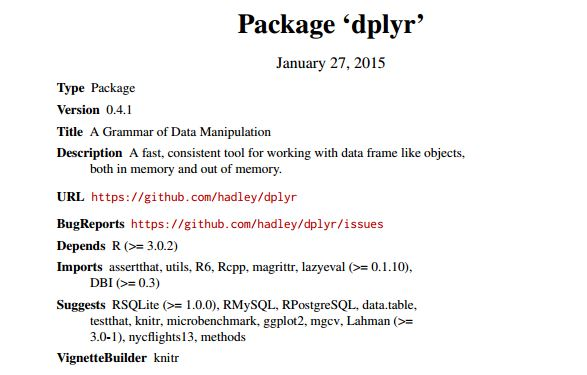
\includegraphics[width=1.05\linewidth]{tenpack00}
		
	\end{figure}
	
\end{frame}
%================================================================ %
\begin{frame}
	\begin{figure}
		\centering
		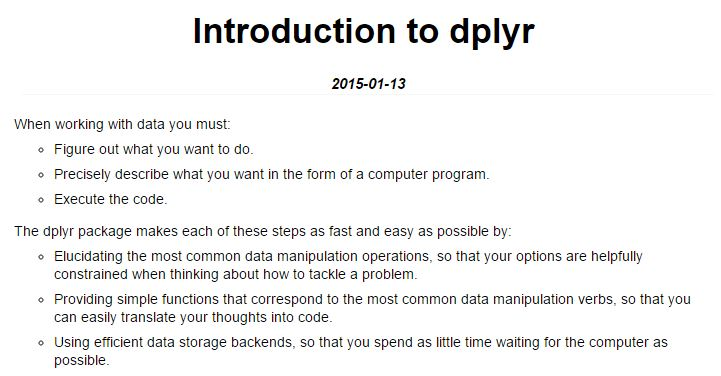
\includegraphics[width=1.15\linewidth]{tenpack01}
		
	\end{figure}
	
\end{frame}
%================================================================ %
\begin{frame}
	\begin{figure}
		\centering
		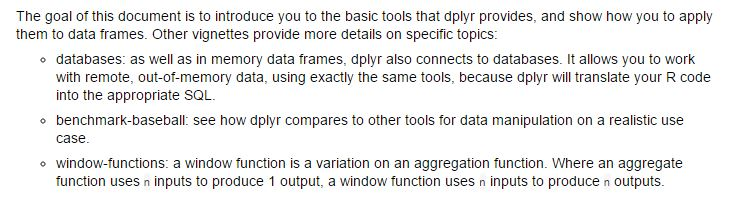
\includegraphics[width=1.15\linewidth]{tenpack02}
		
	\end{figure}
	
\end{frame}

\begin{frame}
\frametitle{magrittr}
\textbf{magrittr: A Forward-Pipe Operator for R}
\begin{itemize}
	\item \textbf{Authors} : Stefan M Bache and Hadley Wickham
\item Provides a mechanism for chaining commands with a new forward-pipe operator, $\%>\%$. 
\item This operator will forward a value, or the result of an expression, into the next function call/expression. 
\item There is flexible support for the type of right-hand side expressions. \item To quote Rene Magritte, "Ceci n'est pas un pipe."
\end{itemize}

\end{frame}
\begin{frame}
	
	\begin{figure}
\centering
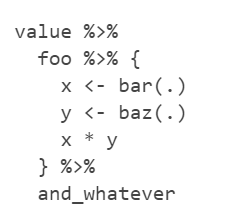
\includegraphics[width=0.99\linewidth]{magrittr}

\end{figure}

\end{frame}
%================================================================ %
\begin{frame}
	\begin{figure}
		\centering
		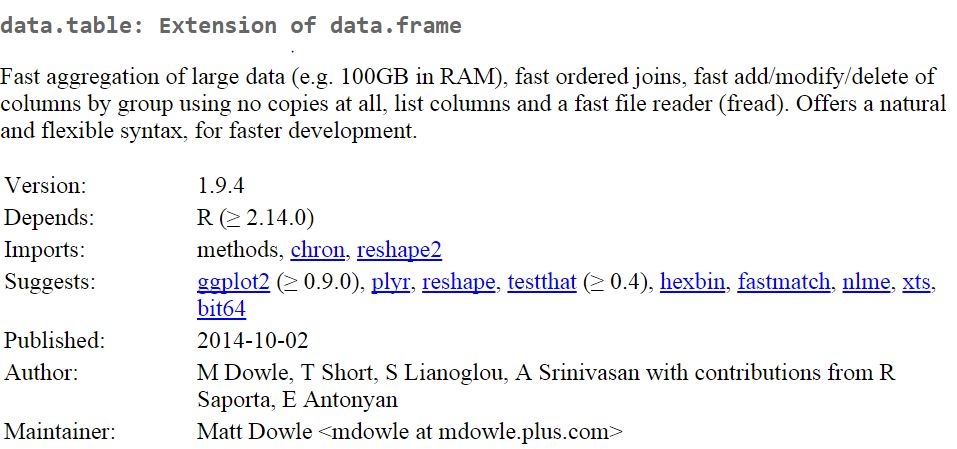
\includegraphics[width=1.15\linewidth]{tenpack03}
		
	\end{figure}
	
\end{frame}
%================================================================ %
\begin{frame}
	\begin{figure}
		\centering
		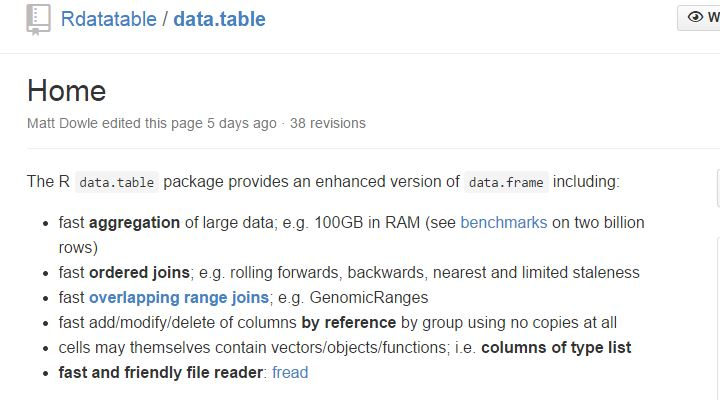
\includegraphics[width=1.15\linewidth]{tenpack04}
		
	\end{figure}
	
\end{frame}

%================================================================ %
\begin{frame}
	\begin{figure}
		\centering
		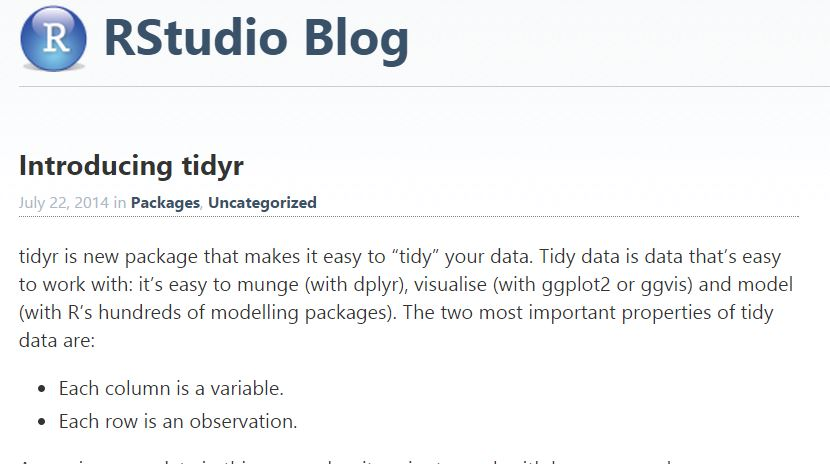
\includegraphics[width=1.15\linewidth]{tidyr}
		
	\end{figure}
	
\end{frame}

\begin{frame}
\begin{quote}
MASS is an amazing package, I always overlook it as well. Maarten-Jan (Kallen, co-developerof Renjin)
made a very interesting point about it too. One of the issues their
particular interpreter has is that they haven't gotten MASS working
for some reason (technical in nature I think) and there are a
phenomenal number of packages that have it as a dependency.

\end{quote}
Michael Cooney - Applied AI Data Scientist
\end{frame}

\end{document}